% !TeX spellcheck = en_US
\documentclass[a4paper,twoside]{article}

\usepackage{epsfig}
\usepackage{subcaption}
\usepackage{calc}
\usepackage{amssymb}
\usepackage{amstext}
\usepackage{amsmath}
\usepackage{amsthm}
\usepackage{multicol}
\usepackage{pslatex}
\usepackage{apalike}
\usepackage{SCITEPRESS}

% user packages
\usepackage{url}

\usepackage{graphicx}
\usepackage{pgfplots}
\pgfplotsset{compat=newest}
\usepackage{colortbl}
\usepackage{xcolor}

\usepackage{listings}
% setup for C and C++
\lstset{
	numbers=left,                   % where to put the line-numbers
	stepnumber=1,                   % the step between two line-numbers.        
	numbersep=3pt,                  % how far the line-numbers are from the code
	numberstyle=\tiny,				% size of the line-numbers
	backgroundcolor=\color{white},  % choose the background color. You must add \usepackage{color}
	showspaces=false,               % show spaces adding particular underscores
	showstringspaces=false,         % underline spaces within strings
	showtabs=false,                 % show tabs within strings adding particular underscores
	tabsize=2,                      % sets default tabsize to 2 spaces
	captionpos=b,                   % sets the caption-position to bottom
	breaklines=true,                % sets automatic line breaking
	breakatwhitespace=true,         % sets if automatic breaks should only happen at whitespace
	title=\lstname,                 % show the filename of files included with \lstinputlisting;
	basicstyle=\ttfamily,			% style of the whole listing
	showstringspaces=false,			% do not show spaces in strings
	keywordstyle=\color{blue}\ttfamily,
	stringstyle=\color{red}\ttfamily,
	commentstyle=\color{teal}\ttfamily\textbf,
}


\begin{document}
	
\title{Exploring DDoS Mechanisms}

\author{\authorname{Bruno de Souza Neves, Filipe Mourão Leite, Lucas da Silva Jorge, Rahyan Azin Gondin Paiva, Juliana de Melo Bezerra and Vitor Venceslau Curtis}
	\affiliation{Department of Computer Science Department, ITA, São José dos Campos, Brazil}
	\email{\{neves.brunobr, filipemleite94, lucas1jorge, rahyan.azin\}@gmail.com, \{juliana, curtis\}@ita.br}
}

\keywords{DDoS, Botnet, Election, Network Topology.}

\abstract{The concern about cyber security has attracted attention by organizations and public services over the last few years due to the contemporary importance of confidentiality, integrity, and availability of services and sensitive data. In contrast, many recent episodes of cyber attacks causing strong impact were performed using extremely simple techniques and taking advantage of the hidden weaknesses of current systems. This article has the main purpose to motivate the academy to mitigate such unexpected potential cyber attacks from the attacker's perspective, exposing the latent weakness of current systems, since the majority of such papers focus only on the defense perspective. We analyze the potential impact of Denial of Service (DoS), a very popular cyber attack to affect the availability of a victim server, through different mechanisms and topologies. Specifically, we simulate and analyze the impact of Distributed DoS (DDoS), a more powerful kind of DDoS, when using the List and Binary Tree topologies with Continuous or Pulsating stream of requests, and finally, we introduce a simple new technique to improve the DDoS against mitigation.
}

\onecolumn \maketitle \normalsize \setcounter{footnote}{0} \vfill

\section{\uppercase{Introduction}}

\noindent Over the last decade, we have seen technologies as streaming, deep learning, IoT, blockchain and big data disrupting traditional business and enabling a prolific market of network-based systems where data are the principal value. In this context, secure and reliable systems are very important to not tarnish the image of a company and crucial in critical systems and public services.

A good example of potential damage a network cyber attack could lead was recently revealed by \cite{McCallie:2011}. They expose the fragility of the Automatic Dependent Surveillance-Broadcast (ADS-B) system of the global air traffic control. Using about \$1,000 worth of radio equipment, a hacker could simply flood the air traffic control system with as many fake airplanes as it wants.

In 2016, Mirai botnet attacked the Internet Service Provider (ISP) for sites such as Twitter, Amazon, PayPal, Spotify, Netflix, and others, making them unreachable for several hours. In such attacks, a worm propagates through networks and systems taking control of poorly protected IoT and embedded devices such as IP cameras, thermostats, Wi-Fi enabled clocks and washing machines \cite{Kolias:2017}. At its peak, Mirai infected over 600,000 vulnerable devices and was able to attack the OVH services with a volume of network traffic around 1Tbps \cite{Antonakakis:2017}.

These episodes expose considerable negligence by companies in the past years regarding security, which now reflects as latent threats to computer systems. Forecastings estimate that IoT and small devices will represent more than 75\% of the global Internet reaching 10 billion in 2020 and representing a true potential threat specially because of new connected solutions with poor security pop up every day by small business and startups, \cite{Rose:2015}, \cite{Columbus:2018}.

With this scenario, we propose that the academy encourage more research papers from the attacker's perspective rather than the defense to force the exposure of current hidden weaknesses of computer systems as a measure of prevention from real potential attacks to organization and states.

According to \cite{Schatz:2017}, the current terminology to discuss security aspects of digital devices and information is cyber security and it is basically defined as the actions and technologies followed by organizations and states to protect confidentiality, integrity, and availability of data and assets used in cyberspace.

Among the cyber threats, the Denial-of-Service (DoS) is a very easy and common kind of cyber attack that violates the availability of systems. Besides it looks harmless at first, as cited by the examples above, it can cause severe damages to organizations and public services. Furthermore, due to the contemporary importance of confidentiality and value of data, cyber attacks can cause an important devaluation of brands by inducing distrust about the integrity and confidentiality of personal data or services, becoming even a tool to commit financial crimes by influencing the stock markets.

In this article, we motivate the attacker's philosophy of cybersecurity by analyzing the performance of some Distributed DoS (DDoS), a non-trivial kind of DoS, as a way to analyze the potential damage a real scenario powered by the growth of IoT devices could cause.

First, we present some basic concepts of DoS and DDoS in section \ref{sec:basic}, followed by a common taxonomy of the main methods of DDoS based on some behavior mechanisms. Section \ref{sec:simulation} describes how to simulate the main methods of DDoS introduced in the previous section and the limitations of these simulations. Section \ref{sec:evaluation} discusses the results of the simulations and the potential of each mechanism. In section \ref{sec:protection}, we propose a new technique difficulting DDoS mitigation by protecting the attacking network and, finally, \ref{sec:conclusion} cites the main conclusions of this work.

\section{\uppercase{Basic concepts of DoS and taxonomy of DDoS}} \label{sec:basic}

DoS is a cyber-attack in which the perpetrator seeks to make a machine or network resource unavailable to its intended users by temporarily or indefinitely disrupting services of a host connected to the Internet \cite{Soltanian:2016}, and it can be achieved by different methods. A simple example of DoS with limited side effect is deliberately entering a wrong password enough consecutive times to cause the victims account to be locked.

Usually, the most common method of attack occurs when the hacker floods a network server or resource with superfluous or incorrect requests in an attempt to decrease its availability to attend legitimate requests and blocking all users at once. One example of such attack is known as SYN flood, where one sends a request to connect but never completes the connection through a three-way handshake. The incomplete handshake leaves the connected port in an occupied status and unavailable for further requests.

Many of these DoS attacks are easy to identify and block by only checking the source of the requests. Because of this, hackers usually use DDoS, which implements distributed computing to coordenate multiple attackers from different sources to send malicious traffic to a targeted server.

\begin{figure}[htb]
	\centering
  \resizebox{0.9\linewidth}{!}{ %\textwidth
  \begin{tikzpicture}[node distance=10mm,
    every node/.style={fill=white, font=\large, minimum width=2.6cm},
    align=center,
    ]
    % retangulo
    \draw[very thin]  (2,1.5) rectangle (6,-7) node[below, xshift=-2cm, yshift=-0.2cm] {Internet devices};
    
    % imagens svg
    \node[label={Hacker}] (hacker) {\includegraphics[scale=1]{"img/standing man icon"}};
    \node[label=below:{C\&C}, right of=hacker, xshift=-1.0cm, yshift=-2.5cm] (cc) {\includegraphics[scale=1]{"img/terminal"}};
    
    \node[right of=cc, xshift=3cm] (infectR) {\includegraphics[scale=0.8]{"img/terminal"}};
    \node[above of=infectR, yshift=0.5cm] (infectA1) {\includegraphics[scale=0.6]{"img/pda"}};
    \node[above of=infectA1, yshift=0.5cm] (infectA2) {\includegraphics[scale=0.8]{"img/RF modem"}};
    \node[below of=infectR, yshift=-0.5cm] (infectB1) {\includegraphics[scale=0.8]{"img/laptop"}};
    \node[label=below:{Infected devices}, below of=infectB1, yshift=-0.5cm] (infectB2) {\includegraphics[scale=0.8]{"img/terminal"}};
    
    \node[label=below:{Company's \\infrastucture}, right of=infectR, xshift=3cm] (router) {\includegraphics[scale=0.9]{"img/router in bldg"}};
    
    % setas
    \draw[<->, thick] (hacker) -- (cc);
    
    \draw[->, dashed, thick] (cc) -- (infectR);
    \draw[->, dashed, thick] (cc) -- (infectA1);
    \draw[<->, thick] (cc) -- (infectA2);
    \draw[red!70, <->, thick] (cc) -- (infectB1);
    \draw[->, dashed, thick] (cc) -- (infectB2);
    
    \draw[<->, thick] (router) -- (infectR);
    \draw[<->, thick] (router) -- (infectA1);
    \draw[<->, thick] (router) -- (infectA2);
    \draw[red!70, <->, thick] (router) -- (infectB1);
    \draw[<->, thick] (router) -- (infectB2);
  \end{tikzpicture}
  }
	\caption{Arquitecture example of a DDoS botnet with one zombie, in red, blocked by the target firewall.}
	\label{fig:DDoS-arch}
\end{figure}

A DDoS starts with the hacker first spreading malicious softwares called malware with the intention to infect an army of Internet-connected devices, named zombie computers, with backdoors running in background and waiting for commands from a Command and Control (C\&C) server, as shown in Figure \ref{fig:DDoS-arch}, configuring a network of zombies called botnet.

After many devices infected, the hacker initiates a DDoS through the C\&C, which is responsible to spread the attack command over the botnet, and each zombie performs the attack by requesting some service over the network to the target infrastructure. It makes the defense much more difficult since blocking one IP, see Figure \ref{fig:DDoS-arch}, has almost no effect because of the massive amount of attacking points spread over the Internet.

DDoS is also much more powerful than a simple DoS because it multiplies the capacity of sending fake request to the target, the massive amount of available resources enables requests with signatures very close to genuine requests, and it can be implemented with no central point of C\&C, making the interruption of an attack much more difficult.

\begin{figure*}[htb]
	\centering
	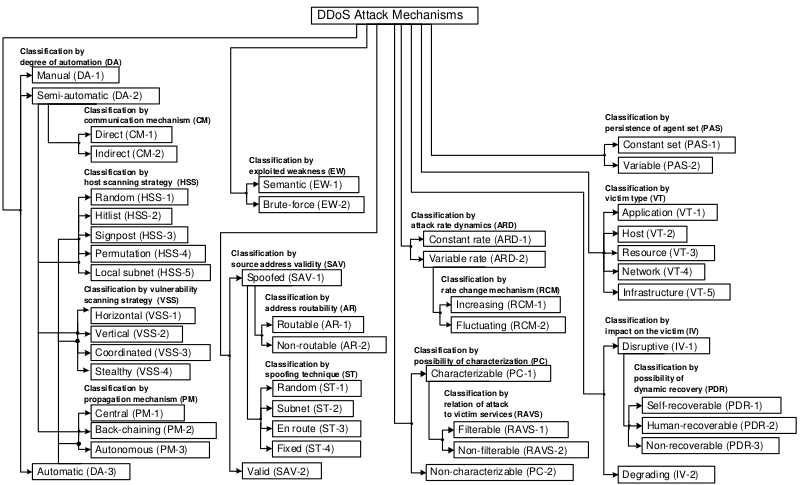
\includegraphics[width=0.9\textwidth]{img/taxonomy}
	\caption{Taxonomy of DDoS attacks.}
	\label{fig:taxonomy}
\end{figure*}

In the literature, there are some taxonomies trying to capture all the methods involving DDoS. \cite{Mirkovic:2004} and \cite{Bhardwaj:2016} classify DDoS attacks by the following main categories: Degree of Automation (DA), Exploited Weakness to Deny Service (EW), Source Address Validity (SAV), Attack Rate Dynamics (ARD), Possibility of Characterization (PC), Persistence of Agent Set (PAS), Victim Type (VT) and Impact on the Victim (IV), as described by Figure \ref{fig:taxonomy}. For more information about the details of this taxonomy and the characteristics of each component, please, see \cite{Mirkovic:2004} and \cite{Bhardwaj:2016}.

According to this classification, our proposed methodology has the following characteristics:
\begin{description}
	\item[Semi-Automatic (DA)] The attack is initiated by the user command, while all the other processes are automatic;
	\item[Brute Force (EW)] It sends a high volume of seemingly legitimate requests to exhaust the victim's capacity;
	\item[Valid Source Address (SAV)] The attacker does not use a spoofed source address;
	\item[Constant or Variable Rate (ARD)] Both dynamics are tested;
	\item[Non-Characterizable (PC)] No specific protocol or application from the victim was chosen to be targeted. The attack only intends to consume network bandwidth;
	\item[Constant Agent Set (PA)] When a node is infected, it becomes a permanent participant in each of the subsequent attacks;
	\item[Network Attack (VT)] The attacks mean to exhaust the bandwidth of a target;
	\item[Disruptive (IV)] The attack has the object to disrupt the entire target's resources, even though sometimes it cannot accomplish it.
\end{description}


Among these characteristics, the Degree of Automation and Attack Rate Dynamics are crucial in our experiments once our goal is to measure the efficiency of a botnet. Thus, the following subsections \ref{sec:da} and \ref{sec:ard} respectively describe in more details the mechanisms of DA and ARD analyzed in our simulations.

\subsection{Degree of automation} \label{sec:da}

%The process of mobilizing zombies and commanding the attack can be either automatic, so that the botnet organizes the process by itself, manual, in which the hacker needs to give most of the commands, or semi-automatic, which is our case. In the methodology applied, the DDoS started through an user input. Then, after initiated, the algorithm kept commanding the attack by itself.

% The semi-automatic degree of automation ... \emph{justificar o modo semi-automático implementado, suas relações com a topologia e apresentar o problema de se esconder a estrutura da rede de zombies para evitar contra-ataque: os zumbies apenas se comunicam com o C\&C durante a fase de ataque. De preferência, adicionar uma diagrama para explicação}.

During the infection of a botnet, the process of infecting new zombies, the dynamic management of the network, and the control of a botnet command may be implemented in different degree of automation \cite{Bhardwaj:2016}:
\begin{description}
	\item[Automatic] Zombie nodes autonomously organize themselves, including a pre-programmed attack pattern;
	\item[Manual] The hacker starts all the commands: attack, network management and infection;
	\item[Semi-automatic] Some degree of automation.
\end{description}

In this work, we preferred the semi-automatic degree of automation once the automatic restricts the flexibility of attack and the manual exposes the botnet network with many control messages. The semi-automatic approach is better once it has all de benefits of common distributed systems: no-central server, resilient to failures, scalable, etc.

Our semi-automatic solution implements a distributed botnet system that dynamically adapts the network, the topology of zombie nodes, once they become available or not due to a new successful infection or mitigation by a security system. Only the start of an attack command is kept manual in order to have more control of the experiments, while the dissemination of any command in the botnet continues autonomously.

Botnets can be formed in different network structures, topologies, for which the most common are:
\begin{description}
	\item[Star topology] There is a C\&C server with the bots organized around it;
	\item[Hierarchical topology] Bots organized in layers of C\&C servers;
	\item[Random topology] Peer-to-peer (P2P) communication	among bots.
\end{description}

The star topology was chosen to facilitate the implementation of the semi-automatic attack, since there is a central server that can receive manual input from a user and then transmit a flow of commands in the direction from the root to leaves.

A weakness of this topology is the possibility of a security system to explore the center of each start. Using this vulnerability, it is possible to reach the C\&C and make it unavailable. In order to avoid this type of mitigation and still preserve the manual control of the attack, in section \ref{sec:protection}, we propose a new method of automation which controls the botnet with resilience, where zombies have only partial information about the topology.

\subsection{Attack rate dynamics} \label{sec:ard}

A DDoS can also follow different dynamics depending on the duration, form, and distribution of the traffic in the stream of superfluous requests, where the more similar its signature is to a genuine request, the more difficult it is to detect the DDoS. A taxonomy with two main classes of ARD patterns are described in \cite{Liu:2012}.

\begin{figure}[htb]
	\centering
	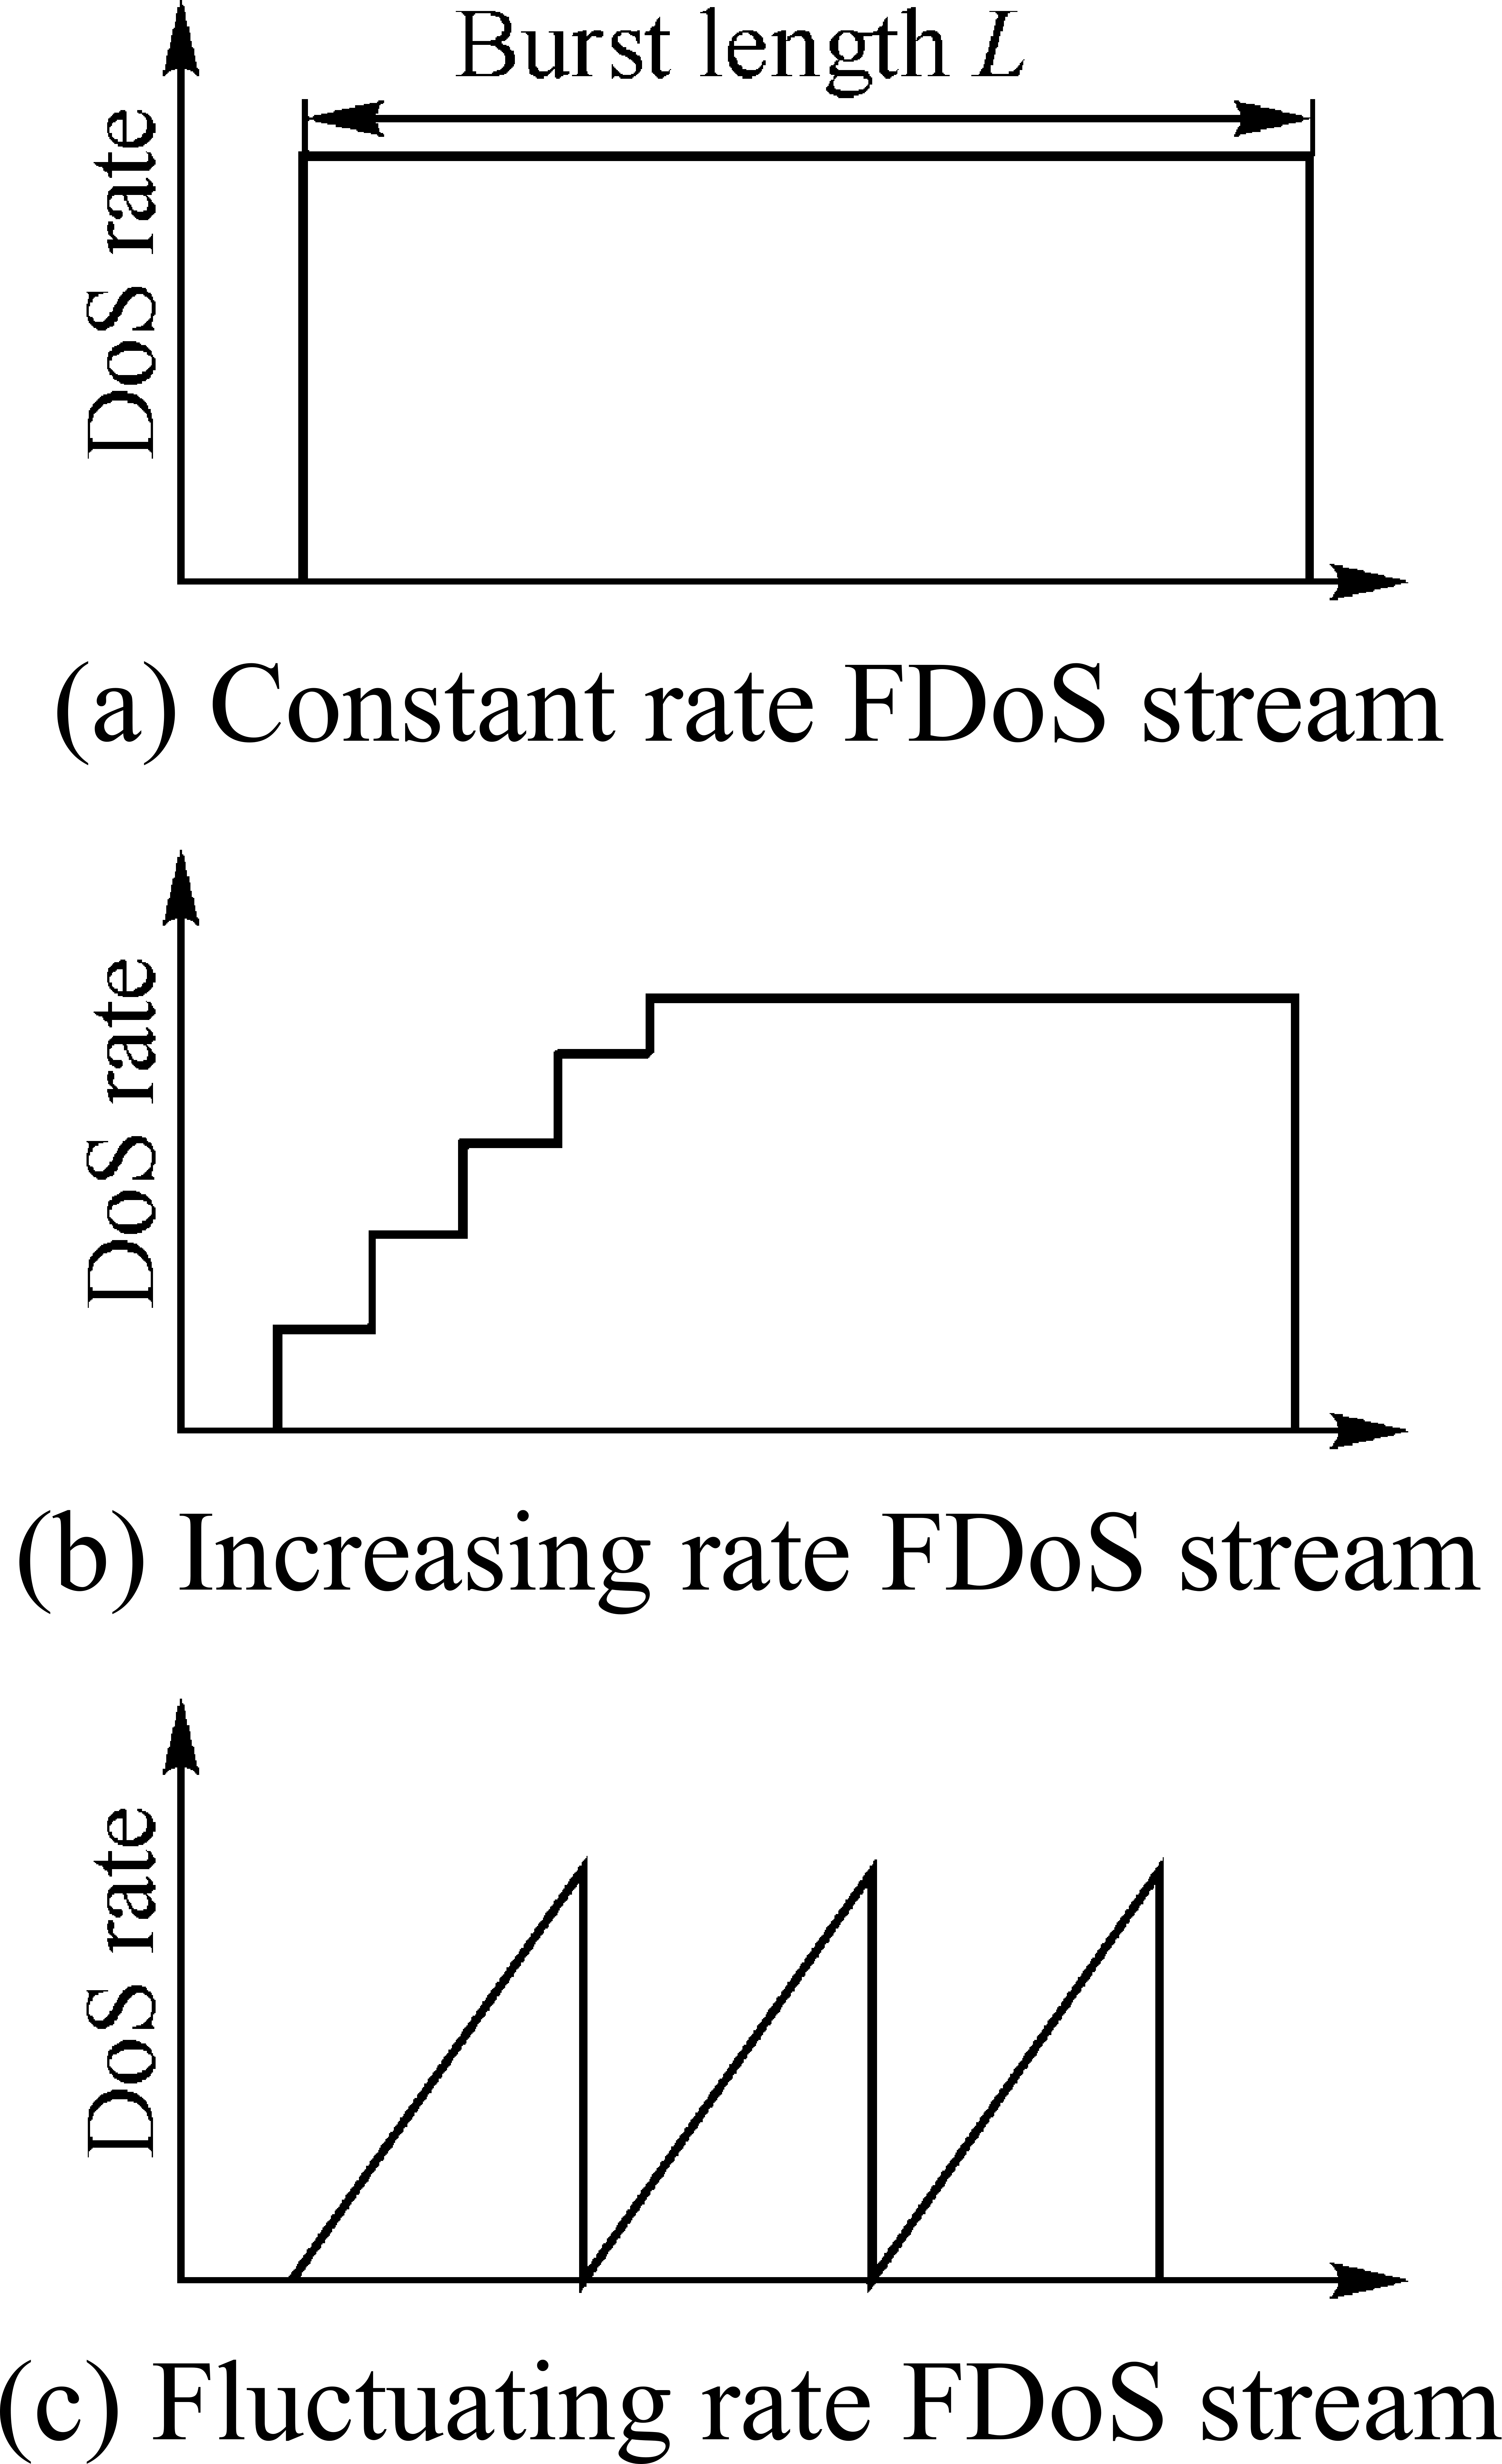
\includegraphics[width=0.5\linewidth]{img/FDoSwaves}
	\caption{Typical FDoS waveforms.}
	\label{fig:fdosWave}
\end{figure}

Flood DoS (FDoS), as showed in Figure \ref{fig:fdosWave}, has three typical types of a waveform based on the ARD: classical constant rate flood, increasing rate flood, fluctuating rate flood. In constant rate, the botnet attacks the target with full force; in increasing rate flood, the botnet gradually increases the attack rate resulting to slow exhaustion of victim's resources; and in fluctuating rate, the botnet performs any other waveform, including occasional changes.

\begin{figure}[htb]
	\centering
	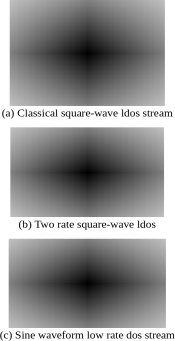
\includegraphics[width=0.6\linewidth]{img/LDoSwaves}
	\caption{Typical LDoS waveforms.}
	\label{fig:ldos}
\end{figure}

Low Rate DoS (LDos) is similar to fluctuating rate flood but it sends just one short burst, usually a square wave pattern, every each $T$ period. For large botnets, $T$ may even be long in order to difficult the detection of the malicious attack. The Figure \ref{fig:ldos} presents some typical different patterns of LDoS.

In this work, we analyze two main patters of a ARD: a continuous stream and a pulse waveform. The first is very similar to the constant rate FDoS and the second is closely related to LDoS pattern. However, it is important to note that the propagation delay of a command from the C\&C into the botnet may drastically change the waveform, resulting in interesting patterns.

\section{\uppercase{Simulations of DDoS}} \label{sec:simulation}

In this work, the two common mechanisms of ARD described in Section \ref{sec:ard} are analyzed, each using two network topologies: a tree-based, where each node in the botnet has some children, and list-based network, where each node can forward an attack only to one next node.

In order to simulate the experiments, we implemented programs in GoLang supported by lightweight threads to achieve a high scale for the botnet simulation. Basically, the simulations are composed by three programs:

\begin{description}
	\item[Server] It is basically the C\&C server, responsible for the botnet commands and for tracking when a node first joined the botnet;
	\item[Client] It is the zombie node, a node in a botnet network, capable of autonomously discovering other zombies and handling attacks;
	\item[Targeted Server] It represents the target infrastructure and stores the attack data for further analysis.
\end{description}

All programs communicate with each other by TCP/IP packages and the Client implements distributed solutions to handle the network topology autonomously. During the simulations, the lost packets to the Target Server are ignored and no information about it is possible to be retrieved from the Target Server. However, it is possible to recover the amount of lost packet by comparing the received packages and the total amount of requests performed by the botnet.

The records about the requests are tagged with timestamps in order to check the time it takes to achieve the target. It is also needed to check the bandwidth capability of each pair of network topology and ARD.

All the codes are available open-source for further researches. Please, contact the authors for getting access to it.

\section{\uppercase{Evaluation of simulations}} \label{sec:evaluation}

This section presents the main results of our simulations for the tree-based and list-based topologies using continuous stream and pulse wave pattern of DDoS attacks. Besides many measurements were obtained from the simulations, we focus in this work only in the package loss once it presents the most representative results of the simulations.

The tests were performed in different machines configurations and the results were all similar. In the following sections, we preferred to show the results from a single common machine configuration.

\subsection{Contamination of zombies}

In a real scenario, a central server of a star topology usually contaminates zombies around it in a tree-like structure. Thus, in order to simulate this approach, we simulate the system in a binary tree topology. Furthermore, to observe the effects of having a large number of levels in the tree architecture with a reasonable number of nodes, we use a botnet with list structure, which in practice is unlikely to happen but it is enough to observe results.

During the contamination phase, for a similar number of nodes, the list-based topology presents a bigger number of layers than a tree-based topology, implying in a larger delay of propagation through the botnet. Because of this, we use 100 nodes for the list implementations. For the binary tree topology, since the height tends to be proportional to $\log_2 n$, we use 500 nodes in the simulation to get more levels and make the effect of the topology clear in the results.

\begin{figure}[bp]
	\centering
	\footnotesize
	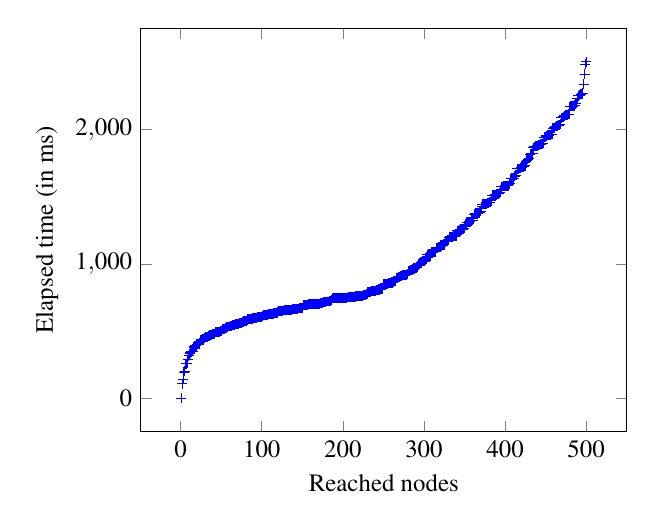
\begin{tikzpicture}[scale=0.9]
	\begin{axis}[
	xlabel=Reached nodes,
	ylabel=Elapsed time (in ms),
	scaled ticks=false,
	xticklabel style={/pgf/number format/fixed}
	]
	%Continuous % binary tree
	\addplot+[only marks, blue, mark=+] plot coordinates {
		(1,0)
		(2,105)
		(3,139)
		(4,191)
		(5,198)
		(6,254)
		(7,254)
		(8,259)
		(9,285)
		(10,315)
		(11,329)
		(12,337)
		(13,343)
		(14,347)
		(15,347)
		(16,378)
		(17,386)
		(18,391)
		(19,391)
		(20,401)
		(21,401)
		(22,401)
		(23,401)
		(24,423)
		(25,429)
		(26,434)
		(27,437)
		(28,437)
		(29,444)
		(30,451)
		(31,453)
		(32,454)
		(33,458)
		(34,461)
		(35,462)
		(36,468)
		(37,469)
		(38,471)
		(39,474)
		(40,474)
		(41,476)
		(42,479)
		(43,489)
		(44,489)
		(45,489)
		(46,491)
		(47,495)
		(48,495)
		(49,501)
		(50,501)
		(51,501)
		(52,513)
		(53,513)
		(54,514)
		(55,522)
		(56,522)
		(57,526)
		(58,531)
		(59,533)
		(60,533)
		(61,535)
		(62,535)
		(63,536)
		(64,541)
		(65,541)
		(66,547)
		(67,547)
		(68,552)
		(69,552)
		(70,554)
		(71,555)
		(72,556)
		(73,556)
		(74,560)
		(75,562)
		(76,563)
		(77,568)
		(78,571)
		(79,572)
		(80,576)
		(81,576)
		(82,582)
		(83,586)
		(84,586)
		(85,589)
		(86,590)
		(87,590)
		(88,591)
		(89,593)
		(90,595)
		(91,595)
		(92,596)
		(93,598)
		(94,600)
		(95,601)
		(96,603)
		(97,603)
		(98,604)
		(99,605)
		(100,607)
		(101,614)
		(102,615)
		(103,616)
		(104,618)
		(105,618)
		(106,619)
		(107,621)
		(108,623)
		(109,623)
		(110,624)
		(111,624)
		(112,627)
		(113,628)
		(114,628)
		(115,633)
		(116,633)
		(117,633)
		(118,634)
		(119,636)
		(120,638)
		(121,647)
		(122,647)
		(123,650)
		(124,651)
		(125,651)
		(126,651)
		(127,652)
		(128,653)
		(129,653)
		(130,653)
		(131,655)
		(132,655)
		(133,655)
		(134,657)
		(135,657)
		(136,657)
		(137,658)
		(138,660)
		(139,660)
		(140,662)
		(141,663)
		(142,663)
		(143,666)
		(144,666)
		(145,667)
		(146,667)
		(147,668)
		(148,670)
		(149,671)
		(150,673)
		(151,691)
		(152,691)
		(153,691)
		(154,692)
		(155,692)
		(156,696)
		(157,696)
		(158,697)
		(159,697)
		(160,699)
		(161,699)
		(162,700)
		(163,700)
		(164,701)
		(165,701)
		(166,702)
		(167,703)
		(168,703)
		(169,703)
		(170,703)
		(171,704)
		(172,706)
		(173,708)
		(174,710)
		(175,711)
		(176,712)
		(177,715)
		(178,716)
		(179,716)
		(180,719)
		(181,719)
		(182,719)
		(183,721)
		(184,721)
		(185,726)
		(186,727)
		(187,742)
		(188,742)
		(189,743)
		(190,743)
		(191,743)
		(192,744)
		(193,744)
		(194,744)
		(195,744)
		(196,744)
		(197,745)
		(198,745)
		(199,745)
		(200,747)
		(201,747)
		(202,747)
		(203,748)
		(204,748)
		(205,748)
		(206,749)
		(207,750)
		(208,750)
		(209,751)
		(210,753)
		(211,753)
		(212,753)
		(213,755)
		(214,756)
		(215,756)
		(216,757)
		(217,757)
		(218,758)
		(219,758)
		(220,758)
		(221,760)
		(222,760)
		(223,760)
		(224,763)
		(225,764)
		(226,765)
		(227,766)
		(228,766)
		(229,772)
		(230,773)
		(231,791)
		(232,791)
		(233,792)
		(234,793)
		(235,794)
		(236,794)
		(237,794)
		(238,794)
		(239,797)
		(240,799)
		(241,802)
		(242,802)
		(243,803)
		(244,805)
		(245,806)
		(246,809)
		(247,809)
		(248,814)
		(249,815)
		(250,847)
		(251,848)
		(252,852)
		(253,852)
		(254,853)
		(255,853)
		(256,857)
		(257,858)
		(258,857)
		(259,857)
		(260,858)
		(261,859)
		(262,861)
		(263,869)
		(264,872)
		(265,872)
		(266,898)
		(267,898)
		(268,900)
		(269,905)
		(270,905)
		(271,907)
		(272,911)
		(273,913)
		(274,915)
		(275,916)
		(276,916)
		(277,916)
		(278,918)
		(279,919)
		(280,921)
		(281,948)
		(282,948)
		(283,951)
		(284,953)
		(285,953)
		(286,959)
		(287,960)
		(288,960)
		(289,967)
		(290,969)
		(291,969)
		(292,973)
		(293,1002)
		(294,1004)
		(295,1004)
		(296,1011)
		(297,1013)
		(298,1018)
		(299,1018)
		(300,1020)
		(301,1020)
		(302,1028)
		(303,1032)
		(304,1069)
		(305,1069)
		(306,1070)
		(307,1073)
		(308,1075)
		(309,1081)
		(310,1083)
		(311,1086)
		(312,1089)
		(313,1089)
		(314,1090)
		(315,1118)
		(316,1119)
		(317,1120)
		(318,1122)
		(319,1123)
		(320,1124)
		(321,1131)
		(322,1135)
		(323,1137)
		(324,1141)
		(325,1141)
		(326,1173)
		(327,1173)
		(328,1173)
		(329,1175)
		(330,1179)
		(331,1198)
		(332,1199)
		(333,1201)
		(334,1202)
		(335,1202)
		(336,1204)
		(337,1204)
		(338,1206)
		(339,1208)
		(340,1209)
		(341,1245)
		(342,1246)
		(343,1248)
		(344,1249)
		(345,1252)
		(346,1255)
		(347,1259)
		(348,1259)
		(349,1262)
		(350,1264)
		(351,1296)
		(352,1296)
		(353,1308)
		(354,1310)
		(355,1311)
		(356,1314)
		(357,1314)
		(358,1321)
		(359,1323)
		(360,1326)
		(361,1334)
		(362,1370)
		(363,1372)
		(364,1375)
		(365,1378)
		(366,1378)
		(367,1378)
		(368,1381)
		(369,1384)
		(370,1393)
		(371,1426)
		(372,1444)
		(373,1444)
		(374,1445)
		(375,1445)
		(376,1446)
		(377,1447)
		(378,1452)
		(379,1453)
		(380,1455)
		(381,1457)
		(382,1458)
		(383,1468)
		(384,1509)
		(385,1511)
		(386,1511)
		(387,1512)
		(388,1514)
		(389,1516)
		(390,1521)
		(391,1522)
		(392,1523)
		(393,1524)
		(394,1534)
		(395,1573)
		(396,1576)
		(397,1576)
		(398,1578)
		(399,1579)
		(400,1580)
		(401,1581)
		(402,1581)
		(403,1582)
		(404,1582)
		(405,1592)
		(406,1595)
		(407,1635)
		(408,1638)
		(409,1639)
		(410,1639)
		(411,1639)
		(412,1652)
		(413,1659)
		(414,1660)
		(415,1708)
		(416,1709)
		(417,1710)
		(418,1710)
		(419,1713)
		(420,1718)
		(421,1720)
		(422,1722)
		(423,1723)
		(424,1731)
		(425,1731)
		(426,1764)
		(427,1771)
		(428,1778)
		(429,1785)
		(430,1786)
		(431,1818)
		(432,1819)
		(433,1819)
		(434,1823)
		(435,1866)
		(436,1874)
		(437,1875)
		(438,1875)
		(439,1878)
		(440,1881)
		(441,1883)
		(442,1884)
		(443,1888)
		(444,1889)
		(445,1895)
		(446,1896)
		(447,1899)
		(448,1943)
		(449,1943)
		(450,1948)
		(451,1954)
		(452,1956)
		(453,1957)
		(454,1957)
		(455,1960)
		(456,1963)
		(457,1967)
		(458,1967)
		(459,2010)
		(460,2015)
		(461,2015)
		(462,2023)
		(463,2024)
		(464,2027)
		(465,2029)
		(466,2032)
		(467,2033)
		(468,2038)
		(469,2088)
		(470,2089)
		(471,2090)
		(472,2097)
		(473,2104)
		(474,2106)
		(475,2109)
		(476,2112)
		(477,2112)
		(478,2113)
		(479,2114)
		(480,2172)
		(481,2173)
		(482,2173)
		(483,2175)
		(484,2175)
		(485,2177)
		(486,2183)
		(487,2193)
		(488,2197)
		(489,2235)
		(490,2251)
		(491,2253)
		(492,2254)
		(493,2263)
		(494,2263)
		(495,2266)
		(496,2270)
		(497,2339)
		(498,2414)
		(499,2487)
		(500,2505)
	};
	\end{axis}
	\end{tikzpicture}
	\normalsize
	\caption{Propagation delay within a botnet with 500 nodes using constant DDoS in binary tree topology.}
	\label{fig:MobContBT}
\end{figure}

\begin{figure}[tbp]
	\centering
	\footnotesize
	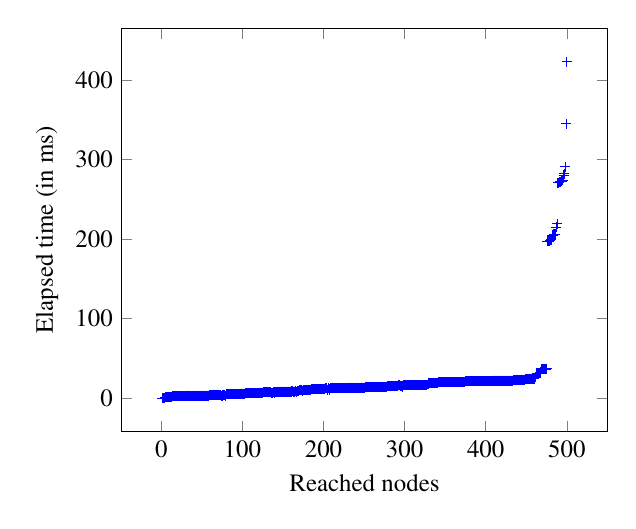
\begin{tikzpicture}[scale=0.9]
	\begin{axis}[
	xlabel=Reached nodes,
	ylabel=Elapsed time (in ms),
	scaled ticks=false,
	xticklabel style={/pgf/number format/fixed}
	]
	%Pulsating % binary tree
	\addplot+[only marks, blue, mark=+] plot coordinates {
		(1,0)
		(2,0)
		(3,0)
		(4,0)
		(5,1)
		(6,1)
		(7,1)
		(8,1)
		(9,1)
		(10,1)
		(11,1)
		(12,1)
		(13,1)
		(14,2)
		(15,2)
		(16,2)
		(17,2)
		(18,2)
		(19,2)
		(20,2)
		(21,2)
		(22,2)
		(23,2)
		(24,2)
		(25,2)
		(26,2)
		(27,2)
		(28,2)
		(29,2)
		(30,2)
		(31,2)
		(32,3)
		(33,3)
		(34,3)
		(35,3)
		(36,3)
		(37,2)
		(38,2)
		(39,2)
		(40,3)
		(41,3)
		(42,3)
		(43,3)
		(44,3)
		(45,3)
		(46,3)
		(47,3)
		(48,3)
		(49,3)
		(50,3)
		(51,3)
		(52,3)
		(53,3)
		(54,3)
		(55,3)
		(56,3)
		(57,3)
		(58,3)
		(59,4)
		(60,4)
		(61,4)
		(62,4)
		(63,4)
		(64,4)
		(65,4)
		(66,4)
		(67,4)
		(68,4)
		(69,4)
		(70,4)
		(71,4)
		(72,4)
		(73,4)
		(74,3)
		(75,4)
		(76,3)
		(77,4)
		(78,4)
		(79,3)
		(80,5)
		(81,5)
		(82,5)
		(83,5)
		(84,5)
		(85,5)
		(86,5)
		(87,5)
		(88,5)
		(89,5)
		(90,5)
		(91,5)
		(92,5)
		(93,5)
		(94,5)
		(95,5)
		(96,5)
		(97,5)
		(98,5)
		(99,5)
		(100,5)
		(101,5)
		(102,5)
		(103,5)
		(104,6)
		(105,6)
		(106,6)
		(107,6)
		(108,6)
		(109,6)
		(110,6)
		(111,6)
		(112,6)
		(113,6)
		(114,6)
		(115,6)
		(116,6)
		(117,6)
		(118,6)
		(119,6)
		(120,6)
		(121,6)
		(122,6)
		(123,6)
		(124,6)
		(125,6)
		(126,7)
		(127,7)
		(128,7)
		(129,7)
		(130,7)
		(131,7)
		(132,7)
		(133,7)
		(134,7)
		(135,7)
		(136,6)
		(137,6)
		(138,7)
		(139,6)
		(140,7)
		(141,7)
		(142,7)
		(143,8)
		(144,8)
		(145,8)
		(146,8)
		(147,8)
		(148,8)
		(149,8)
		(150,8)
		(151,8)
		(152,8)
		(153,8)
		(154,8)
		(155,8)
		(156,8)
		(157,8)
		(158,8)
		(159,8)
		(160,9)
		(161,8)
		(162,9)
		(163,8)
		(164,8)
		(165,9)
		(166,9)
		(167,8)
		(168,9)
		(169,9)
		(170,10)
		(171,10)
		(172,10)
		(173,10)
		(174,9)
		(175,10)
		(176,10)
		(177,10)
		(178,10)
		(179,10)
		(180,10)
		(181,10)
		(182,10)
		(183,10)
		(184,10)
		(185,11)
		(186,11)
		(187,11)
		(188,11)
		(189,11)
		(190,11)
		(191,11)
		(192,11)
		(193,11)
		(194,11)
		(195,11)
		(196,11)
		(197,11)
		(198,11)
		(199,11)
		(200,11)
		(201,11)
		(202,12)
		(203,12)
		(204,12)
		(205,10)
		(206,12)
		(207,10)
		(208,11)
		(209,12)
		(210,12)
		(211,12)
		(212,12)
		(213,12)
		(214,12)
		(215,12)
		(216,12)
		(217,12)
		(218,12)
		(219,12)
		(220,12)
		(221,12)
		(222,12)
		(223,12)
		(224,12)
		(225,12)
		(226,12)
		(227,12)
		(228,12)
		(229,12)
		(230,13)
		(231,13)
		(232,13)
		(233,13)
		(234,13)
		(235,13)
		(236,13)
		(237,13)
		(238,13)
		(239,13)
		(240,13)
		(241,13)
		(242,13)
		(243,13)
		(244,13)
		(245,13)
		(246,13)
		(247,13)
		(248,13)
		(249,13)
		(250,12)
		(251,13)
		(252,14)
		(253,14)
		(254,14)
		(255,14)
		(256,14)
		(257,14)
		(258,14)
		(259,14)
		(260,14)
		(261,14)
		(262,14)
		(263,14)
		(264,14)
		(265,14)
		(266,14)
		(267,14)
		(268,14)
		(269,14)
		(270,14)
		(271,14)
		(272,14)
		(273,14)
		(274,14)
		(275,14)
		(276,14)
		(277,14)
		(278,14)
		(279,15)
		(280,15)
		(281,15)
		(282,15)
		(283,15)
		(284,15)
		(285,15)
		(286,15)
		(287,15)
		(288,15)
		(289,15)
		(290,15)
		(291,15)
		(292,16)
		(293,16)
		(294,16)
		(295,15)
		(296,15)
		(297,15)
		(298,14)
		(299,16)
		(300,16)
		(301,16)
		(302,16)
		(303,16)
		(304,16)
		(305,16)
		(306,16)
		(307,16)
		(308,16)
		(309,16)
		(310,16)
		(311,16)
		(312,16)
		(313,16)
		(314,16)
		(315,16)
		(316,16)
		(317,16)
		(318,16)
		(319,16)
		(320,16)
		(321,16)
		(322,16)
		(323,16)
		(324,16)
		(325,16)
		(326,16)
		(327,16)
		(328,17)
		(329,17)
		(330,19)
		(331,19)
		(332,19)
		(333,19)
		(334,19)
		(335,19)
		(336,19)
		(337,19)
		(338,19)
		(339,19)
		(340,19)
		(341,19)
		(342,20)
		(343,20)
		(344,20)
		(345,20)
		(346,20)
		(347,20)
		(348,20)
		(349,20)
		(350,20)
		(351,20)
		(352,20)
		(353,20)
		(354,20)
		(355,20)
		(356,20)
		(357,20)
		(358,20)
		(359,20)
		(360,20)
		(361,20)
		(362,20)
		(363,20)
		(364,20)
		(365,20)
		(366,20)
		(367,20)
		(368,20)
		(369,20)
		(370,20)
		(371,20)
		(372,20)
		(373,20)
		(374,20)
		(375,21)
		(376,21)
		(377,21)
		(378,21)
		(379,21)
		(380,21)
		(381,21)
		(382,21)
		(383,21)
		(384,21)
		(385,21)
		(386,21)
		(387,21)
		(388,21)
		(389,21)
		(390,21)
		(391,21)
		(392,21)
		(393,21)
		(394,21)
		(395,21)
		(396,21)
		(397,21)
		(398,21)
		(399,21)
		(400,21)
		(401,21)
		(402,21)
		(403,21)
		(404,21)
		(405,21)
		(406,21)
		(407,21)
		(408,22)
		(409,22)
		(410,22)
		(411,22)
		(412,22)
		(413,22)
		(414,22)
		(415,22)
		(416,22)
		(417,22)
		(418,22)
		(419,22)
		(420,22)
		(421,22)
		(422,22)
		(423,22)
		(424,22)
		(425,22)
		(426,22)
		(427,22)
		(428,22)
		(429,22)
		(430,22)
		(431,22)
		(432,22)
		(433,22)
		(434,23)
		(435,23)
		(436,23)
		(437,23)
		(438,23)
		(439,23)
		(440,23)
		(441,23)
		(442,23)
		(443,23)
		(444,23)
		(445,23)
		(446,23)
		(447,23)
		(448,23)
		(449,24)
		(450,24)
		(451,24)
		(452,24)
		(453,24)
		(454,24)
		(455,24)
		(456,24)
		(457,24)
		(458,24)
		(459,24)
		(460,24)
		(461,26)
		(462,30)
		(463,31)
		(464,31)
		(465,31)
		(466,31)
		(467,31)
		(468,33)
		(469,36)
		(470,36)
		(471,36)
		(472,36)
		(473,36)
		(474,36)
		(475,37)
		(476,197)
		(477,197)
		(478,197)
		(479,198)
		(480,199)
		(481,199)
		(482,205)
		(483,205)
		(484,206)
		(485,206)
		(486,206)
		(487,215)
		(488,219)
		(489,271)
		(490,271)
		(491,272)
		(492,272)
		(493,273)
		(494,273)
		(495,274)
		(496,280)
		(497,282)
		(498,291)
		(499,345)
		(500,423)
	};
	\end{axis}
	\end{tikzpicture}
	\normalsize
	\caption{Propagation delay within a botnet with 500 nodes using pulse DDoS in binary tree topology.}
	\label{fig:MobPulBT}
\end{figure}

\begin{figure}[tbp]
	\centering
	\footnotesize
	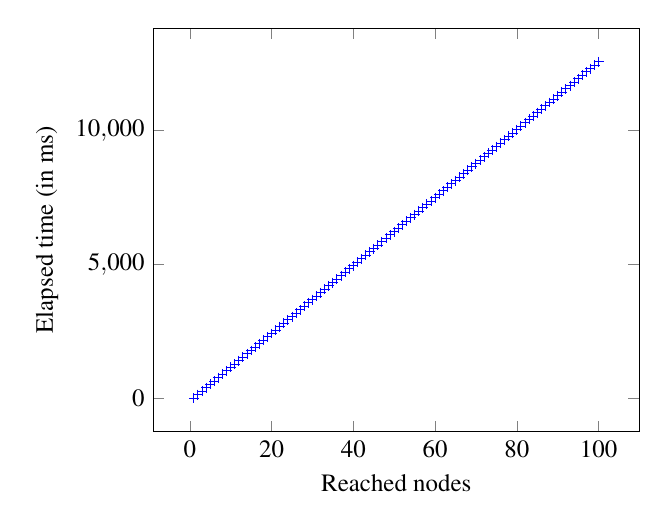
\begin{tikzpicture}[scale=0.9]
	\begin{axis}[
	xlabel=Reached nodes,
	ylabel=Elapsed time (in ms),
	scaled ticks=false,
	xticklabel style={/pgf/number format/fixed}
	]
	%Continuous % List
	\addplot+[only marks, blue, mark=+] plot coordinates {
		(1,0)
		(2,127)
		(3,254)
		(4,381)
		(5,507)
		(6,634)
		(7,761)
		(8,888)
		(9,1014)
		(10,1141)
		(11,1267)
		(12,1394)
		(13,1521)
		(14,1648)
		(15,1774)
		(16,1901)
		(17,2027)
		(18,2154)
		(19,2280)
		(20,2408)
		(21,2534)
		(22,2661)
		(23,2788)
		(24,2915)
		(25,3040)
		(26,3167)
		(27,3293)
		(28,3422)
		(29,3548)
		(30,3674)
		(31,3800)
		(32,3927)
		(33,4054)
		(34,4182)
		(35,4310)
		(36,4435)
		(37,4562)
		(38,4688)
		(39,4818)
		(40,4945)
		(41,5071)
		(42,5198)
		(43,5325)
		(44,5451)
		(45,5578)
		(46,5705)
		(47,5831)
		(48,5958)
		(49,6085)
		(50,6213)
		(51,6340)
		(52,6466)
		(53,6592)
		(54,6720)
		(55,6846)
		(56,6973)
		(57,7099)
		(58,7226)
		(59,7352)
		(60,7480)
		(61,7608)
		(62,7734)
		(63,7862)
		(64,7988)
		(65,8114)
		(66,8242)
		(67,8369)
		(68,8496)
		(69,8623)
		(70,8750)
		(71,8876)
		(72,9003)
		(73,9130)
		(74,9256)
		(75,9383)
		(76,9510)
		(77,9636)
		(78,9763)
		(79,9890)
		(80,10016)
		(81,10143)
		(82,10270)
		(83,10396)
		(84,10523)
		(85,10650)
		(86,10776)
		(87,10903)
		(88,11029)
		(89,11156)
		(90,11283)
		(91,11409)
		(92,11536)
		(93,11663)
		(94,11789)
		(95,11916)
		(96,12043)
		(97,12169)
		(98,12296)
		(99,12423)
		(100,12549)
	};
	\end{axis}
	\end{tikzpicture}
	\normalsize
	\caption{Propagation delay within a botnet with 100 nodes using constant DDoS in list topology.}
	\label{fig:MobContL}
\end{figure}

\begin{figure}[tbp]
	\centering
	\footnotesize
	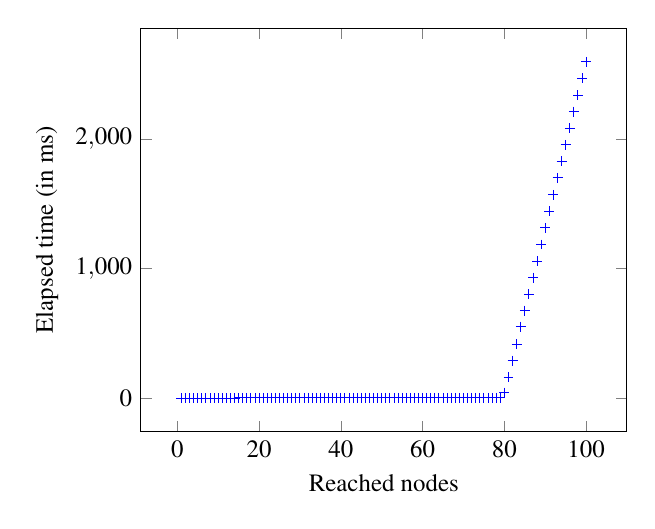
\begin{tikzpicture}[scale=0.9]
	\begin{axis}[
	xlabel=Reached nodes,
	ylabel=Elapsed time (in ms),
	scaled ticks=false,
	xticklabel style={/pgf/number format/fixed}
	]
	%Pulsating % List
	\addplot+[only marks, blue, mark=+] plot coordinates {
		(1,0)
		(2,0)
		(3,0)
		(4,0)
		(5,0)
		(6,0)
		(7,0)
		(8,0)
		(9,0)
		(10,0)
		(11,0)
		(12,0)
		(13,0)
		(14,0)
		(15,1)
		(16,1)
		(17,1)
		(18,1)
		(19,1)
		(20,1)
		(21,1)
		(22,1)
		(23,1)
		(24,1)
		(25,1)
		(26,1)
		(27,1)
		(28,1)
		(29,1)
		(30,1)
		(31,1)
		(32,1)
		(33,1)
		(34,1)
		(35,1)
		(36,1)
		(37,1)
		(38,1)
		(39,1)
		(40,1)
		(41,1)
		(42,1)
		(43,1)
		(44,1)
		(45,1)
		(46,1)
		(47,1)
		(48,1)
		(49,1)
		(50,1)
		(51,1)
		(52,1)
		(53,1)
		(54,1)
		(55,1)
		(56,1)
		(57,1)
		(58,1)
		(59,1)
		(60,1)
		(61,1)
		(62,1)
		(63,1)
		(64,1)
		(65,1)
		(66,1)
		(67,1)
		(68,1)
		(69,1)
		(70,1)
		(71,1)
		(72,1)
		(73,1)
		(74,1)
		(75,1)
		(76,1)
		(77,1)
		(78,1)
		(79,1)
		(80,42)
		(81,161)
		(82,289)
		(83,417)
		(84,551)
		(85,674)
		(86,801)
		(87,930)
		(88,1057)
		(89,1185)
		(90,1314)
		(91,1442)
		(92,1568)
		(93,1699)
		(94,1826)
		(95,1953)
		(96,2082)
		(97,2211)
		(98,2338)
		(99,2469)
		(100,2595)
	};
	\end{axis}
	\end{tikzpicture}
	\normalsize
	\caption{Propagation delay within a botnet with 100 nodes using pulse DDoS in list topology.}
	\label{fig:MobPulL}
\end{figure}

The results are presented in Figures \ref{fig:MobContBT}-\ref{fig:MobPulL}, and it is important to highlight that the graphs are in the same scale in order to make the shape of curves more evident.

Using pulse DDoS mechanism, Figure \ref{fig:MobPulBT} and Figure \ref{fig:MobPulL}, it can be noticed that almost all nodes attack at the same time, delay near $0$ms, except for outliers that do not attack immediately for some unexpected fail or oscillation, a phenomena also present in a real network.

The graphs of the constant DDoS mechanism, Figure \ref{fig:MobContBT} and Figure \ref{fig:MobContL}, show how the nodes are gradually mobilized by the attack wave, exposing the hierarchy of a network with many layers. Particularly, the propagation delay using constant DDoS and list topology, Figure \ref{fig:MobContL}, results in perfect straight line once the information in the list is passed from node to node with a similar delay.


\subsection{Package loss in target server}

\begin{figure}[bp]
	\centering
	\footnotesize
	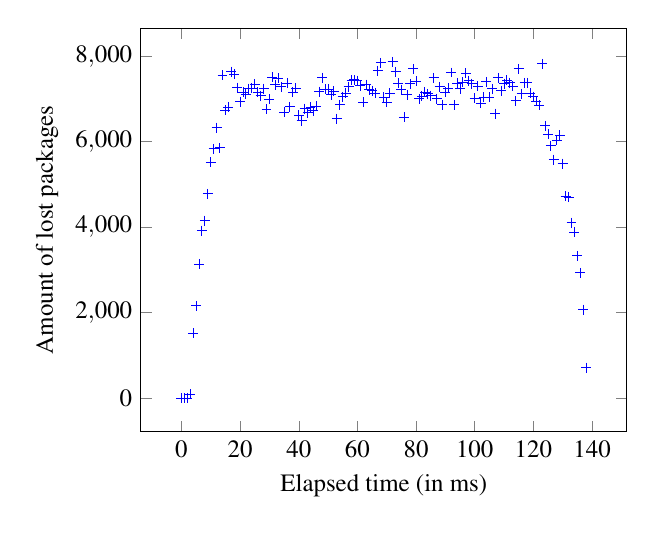
\begin{tikzpicture}[scale=0.9]
	\begin{axis}[
	xlabel=Elapsed time (in ms),
	ylabel=Amount of lost packages,
	scaled ticks=false,
	xticklabel style={/pgf/number format/fixed}
	]
	%Continuous & binary tree
	\addplot+[only marks, blue, mark=+] plot coordinates {
		(0,0)
		(1,0)
		(2,0)
		(3,88)
		(4,1515)
		(5,2155)
		(6,3127)
		(7,3917)
		(8,4153)
		(9,4775)
		(10,5516)
		(11,5828)
		(12,6329)
		(13,5854)
		(14,7548)
		(15,6731)
		(16,6809)
		(17,7636)
		(18,7578)
		(19,7265)
		(20,6936)
		(21,7153)
		(22,7105)
		(23,7237)
		(24,7251)
		(25,7338)
		(26,7151)
		(27,7077)
		(28,7241)
		(29,6761)
		(30,6991)
		(31,7511)
		(32,7332)
		(33,7477)
		(34,7278)
		(35,6691)
		(36,7365)
		(37,6814)
		(38,7160)
		(39,7246)
		(40,6618)
		(41,6490)
		(42,6769)
		(43,6673)
		(44,6804)
		(45,6722)
		(46,6823)
		(47,7168)
		(48,7498)
		(49,7229)
		(50,7227)
		(51,7097)
		(52,7183)
		(53,6535)
		(54,6860)
		(55,7048)
		(56,7133)
		(57,7286)
		(58,7435)
		(59,7441)
		(60,7426)
		(61,7308)
		(62,6922)
		(63,7336)
		(64,7217)
		(65,7191)
		(66,7131)
		(67,7662)
		(68,7841)
		(69,7042)
		(70,6925)
		(71,7128)
		(72,7867)
		(73,7634)
		(74,7369)
		(75,7217)
		(76,6571)
		(77,7095)
		(78,7353)
		(79,7703)
		(80,7408)
		(81,7001)
		(82,7066)
		(83,7150)
		(84,7117)
		(85,7077)
		(86,7494)
		(87,6998)
		(88,7282)
		(89,6866)
		(90,7160)
		(91,7251)
		(92,7616)
		(93,6860)
		(94,7361)
		(95,7241)
		(96,7391)
		(97,7603)
		(98,7426)
		(99,7355)
		(100,7011)
		(101,7299)
		(102,6902)
		(103,7038)
		(104,7395)
		(105,7037)
		(106,7233)
		(107,6653)
		(108,7489)
		(109,7190)
		(110,7355)
		(111,7436)
		(112,7379)
		(113,7296)
		(114,6953)
		(115,7699)
		(116,7118)
		(117,7372)
		(118,7375)
		(119,7132)
		(120,7051)
		(121,6946)
		(122,6851)
		(123,7818)
		(124,6370)
		(125,6175)
		(126,5899)
		(127,5578)
		(128,6026)
		(129,6143)
		(130,5483)
		(131,4725)
		(132,4700)
		(133,4102)
		(134,3881)
		(135,3327)
		(136,2926)
		(137,2070)
		(138,712)
	};
	\end{axis}
	\end{tikzpicture}
	\normalsize
	\caption{Package loss for each ten thousand packages using constant DDoS in Binary Tree topology.}
	\label{fig:ContBinTree}
\end{figure}

\begin{figure}[btp]
	\centering
	\footnotesize
	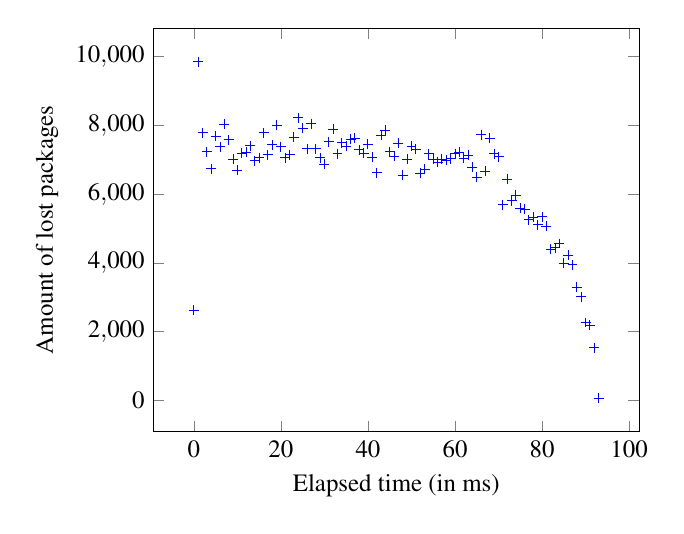
\begin{tikzpicture}[scale=0.9]
	\begin{axis}[
	xlabel=Elapsed time (in ms),
	ylabel=Amount of lost packages,
	scaled ticks=false,
	xticklabel style={/pgf/number format/fixed}
	]
	%Pulsating & binary tree
	\addplot+[only marks, blue, mark=+] plot coordinates {
		(0,2630)
		(1,9844)
		(2,7783)
		(3,7223)
		(4,6733)
		(5,7677)
		(6,7371)
		(7,8036)
		(8,7575)
		(9,7013)
		(10,6698)
		(11,7189)
		(12,7222)
		(13,7403)
		(14,6962)
		(15,7056)
		(16,7783)
		(17,7141)
		(18,7432)
		(19,8002)
		(20,7379)
		(21,7051)
		(22,7149)
		(23,7657)
		(24,8217)
		(25,7907)
		(26,7318)
		(27,8044)
		(28,7314)
		(29,7060)
		(30,6861)
		(31,7521)
		(32,7883)
		(33,7172)
		(34,7490)
		(35,7390)
		(36,7591)
		(37,7625)
		(38,7284)
		(39,7189)
		(40,7452)
		(41,7067)
		(42,6614)
		(43,7711)
		(44,7848)
		(45,7229)
		(46,7103)
		(47,7481)
		(48,6544)
		(49,7013)
		(50,7396)
		(51,7301)
		(52,6607)
		(53,6728)
		(54,7177)
		(55,7013)
		(56,6931)
		(57,7007)
		(58,6984)
		(59,7022)
		(60,7168)
		(61,7217)
		(62,7037)
		(63,7134)
		(64,6784)
		(65,6489)
		(66,7730)
		(67,6670)
		(68,7622)
		(69,7178)
		(70,7081)
		(71,5694)
		(72,6431)
		(73,5807)
		(74,5963)
		(75,5584)
		(76,5555)
		(77,5259)
		(78,5332)
		(79,5110)
		(80,5336)
		(81,5059)
		(82,4390)
		(83,4443)
		(84,4564)
		(85,3994)
		(86,4226)
		(87,3943)
		(88,3292)
		(89,3020)
		(90,2268)
		(91,2182)
		(92,1535)
		(93,74)
	};
	\end{axis}
	\end{tikzpicture}
	\normalsize
	\caption{Package loss for each ten thousand packages using pulse DDoS in Binary Tree topology.}
	\label{fig:PulBinTree}
\end{figure}

\begin{figure}[btp]
	\centering
	\footnotesize
	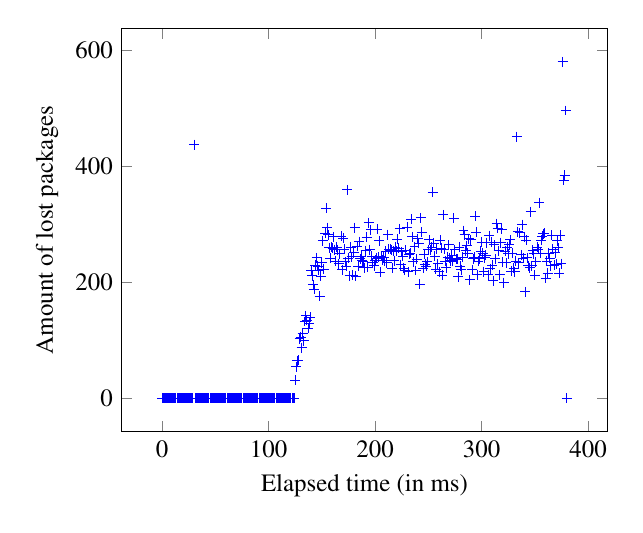
\begin{tikzpicture}[scale=0.9]
	\begin{axis}[
	xlabel=Elapsed time (in ms),
	ylabel=Amount of lost packages,
	scaled ticks=false,
	xticklabel style={/pgf/number format/fixed}
	]
	%Continuous & list
	\addplot+[only marks, blue, mark=+] plot coordinates {
		(0,0)
		(1,0)
		(2,0)
		(3,0)
		(4,0)
		(5,0)
		(6,0)
		(7,0)
		(8,0)
		(9,0)
		(10,0)
		(11,0)
		(12,0)
		(13,0)
		(14,0)
		(15,0)
		(16,0)
		(17,0)
		(18,0)
		(19,0)
		(20,0)
		(21,0)
		(22,0)
		(23,0)
		(24,0)
		(25,0)
		(26,0)
		(27,0)
		(28,0)
		(29,0)
		(30,437)
		(31,0)
		(32,0)
		(33,0)
		(34,0)
		(35,0)
		(36,0)
		(37,0)
		(38,0)
		(39,0)
		(40,0)
		(41,0)
		(42,0)
		(43,0)
		(44,0)
		(45,0)
		(46,0)
		(47,0)
		(48,0)
		(49,0)
		(50,0)
		(51,0)
		(52,0)
		(53,0)
		(54,0)
		(55,0)
		(56,0)
		(57,0)
		(58,0)
		(59,0)
		(60,0)
		(61,0)
		(62,0)
		(63,0)
		(64,0)
		(65,0)
		(66,0)
		(67,0)
		(68,0)
		(69,0)
		(70,0)
		(71,0)
		(72,0)
		(73,0)
		(74,0)
		(75,0)
		(76,0)
		(77,0)
		(78,0)
		(79,0)
		(80,0)
		(81,0)
		(82,0)
		(83,0)
		(84,0)
		(85,0)
		(86,0)
		(87,0)
		(88,0)
		(89,0)
		(90,0)
		(91,0)
		(92,0)
		(93,0)
		(94,0)
		(95,0)
		(96,0)
		(97,0)
		(98,0)
		(99,0)
		(100,0)
		(101,0)
		(102,0)
		(103,0)
		(104,0)
		(105,0)
		(106,0)
		(107,0)
		(108,0)
		(109,0)
		(110,0)
		(111,0)
		(112,0)
		(113,0)
		(114,0)
		(115,0)
		(116,0)
		(117,0)
		(118,0)
		(119,0)
		(120,0)
		(121,0)
		(122,0)
		(123,0)
		(124,0)
		(125,31)
		(126,54)
		(127,64)
		(128,65)
		(129,102)
		(130,105)
		(131,87)
		(132,112)
		(133,99)
		(134,132)
		(135,142)
		(136,134)
		(137,120)
		(138,129)
		(139,139)
		(140,220)
		(141,211)
		(142,195)
		(143,188)
		(144,229)
		(145,242)
		(146,227)
		(147,220)
		(148,176)
		(149,210)
		(150,233)
		(151,271)
		(152,222)
		(153,284)
		(154,327)
		(155,294)
		(156,282)
		(157,259)
		(158,241)
		(159,260)
		(160,258)
		(161,278)
		(162,256)
		(163,236)
		(164,260)
		(165,256)
		(166,232)
		(167,249)
		(168,279)
		(169,221)
		(170,276)
		(171,257)
		(172,235)
		(173,227)
		(174,359)
		(175,241)
		(176,211)
		(177,260)
		(178,244)
		(179,212)
		(180,251)
		(181,294)
		(182,210)
		(183,262)
		(184,227)
		(185,270)
		(186,240)
		(187,245)
		(188,237)
		(189,235)
		(190,225)
		(191,254)
		(192,277)
		(193,226)
		(194,302)
		(195,256)
		(196,290)
		(197,245)
		(198,233)
		(199,228)
		(200,238)
		(201,241)
		(202,291)
		(203,243)
		(204,271)
		(205,217)
		(206,245)
		(207,238)
		(208,243)
		(209,237)
		(210,253)
		(211,233)
		(212,282)
		(213,257)
		(214,257)
		(215,255)
		(216,224)
		(217,253)
		(218,237)
		(219,260)
		(220,254)
		(221,274)
		(222,258)
		(223,292)
		(224,230)
		(225,252)
		(226,245)
		(227,224)
		(228,220)
		(229,255)
		(230,295)
		(231,218)
		(232,248)
		(233,250)
		(234,308)
		(235,278)
		(236,235)
		(237,261)
		(238,220)
		(239,239)
		(240,275)
		(241,267)
		(242,196)
		(243,311)
		(244,286)
		(245,224)
		(246,248)
		(247,231)
		(248,227)
		(249,235)
		(250,256)
		(251,273)
		(252,256)
		(253,260)
		(254,355)
		(255,267)
		(256,245)
		(257,222)
		(258,257)
		(259,232)
		(260,218)
		(261,272)
		(262,258)
		(263,212)
		(264,316)
		(265,257)
		(266,236)
		(267,225)
		(268,243)
		(269,264)
		(270,241)
		(271,237)
		(272,246)
		(273,236)
		(274,310)
		(275,256)
		(276,240)
		(277,239)
		(278,209)
		(279,260)
		(280,227)
		(281,221)
		(282,243)
		(283,289)
		(284,282)
		(285,254)
		(286,263)
		(287,250)
		(288,275)
		(289,204)
		(290,273)
		(291,221)
		(292,240)
		(293,243)
		(294,314)
		(295,286)
		(296,213)
		(297,236)
		(298,240)
		(299,253)
		(300,269)
		(301,250)
		(302,218)
		(303,242)
		(304,246)
		(305,268)
		(306,213)
		(307,280)
		(308,223)
		(309,269)
		(310,229)
		(311,202)
		(312,264)
		(313,240)
		(314,301)
		(315,293)
		(316,254)
		(317,213)
		(318,268)
		(319,291)
		(320,234)
		(321,199)
		(322,253)
		(323,233)
		(324,260)
		(325,249)
		(326,264)
		(327,273)
		(328,219)
		(329,250)
		(330,224)
		(331,218)
		(332,236)
		(333,451)
		(334,287)
		(335,233)
		(336,285)
		(337,247)
		(338,299)
		(339,241)
		(340,278)
		(341,183)
		(342,272)
		(343,242)
		(344,228)
		(345,225)
		(346,321)
		(347,228)
		(348,255)
		(349,249)
		(350,212)
		(351,235)
		(352,260)
		(353,257)
		(354,337)
		(355,250)
		(356,272)
		(357,279)
		(358,283)
		(359,284)
		(360,207)
		(361,236)
		(362,215)
		(363,250)
		(364,241)
		(365,228)
		(366,281)
		(367,257)
		(368,229)
		(369,251)
		(370,231)
		(371,271)
		(372,259)
		(373,215)
		(374,281)
		(375,232)
		(376,580)
		(377,376)
		(378,384)
		(379,496)
		(380,0)
	};
	\end{axis}
	\end{tikzpicture}
	\normalsize
	\caption{Package loss for each ten thousand packages using constant DDoS in List topology.}
	\label{fig:ContList}
\end{figure}

\begin{figure}[btp]
	\centering
	\footnotesize
	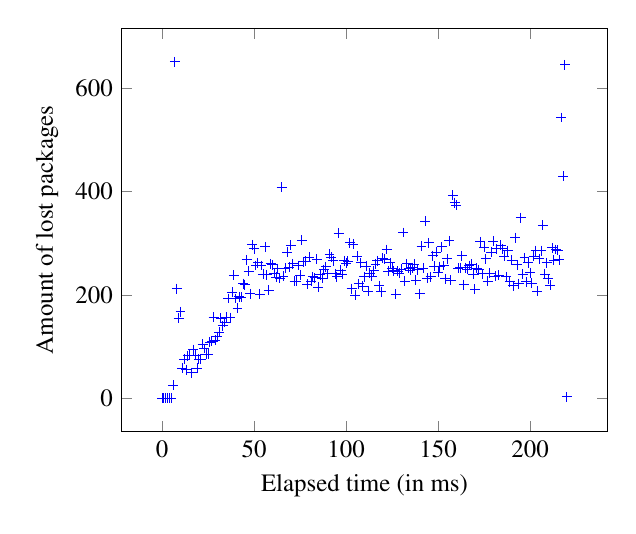
\begin{tikzpicture}[scale=0.9]
	\begin{axis}[
	xlabel=Elapsed time (in ms),
	ylabel=Amount of lost packages,
	scaled ticks=false,
	xticklabel style={/pgf/number format/fixed}
	]
	%Pulsating & list
	\addplot+[only marks, blue, mark=+] plot coordinates {
		(0,0)
		(1,0)
		(2,0)
		(3,0)
		(4,0)
		(5,0)
		(6,25)
		(7,652)
		(8,212)
		(9,155)
		(10,167)
		(11,58)
		(12,75)
		(13,55)
		(14,82)
		(15,83)
		(16,49)
		(17,94)
		(18,83)
		(19,58)
		(20,75)
		(21,75)
		(22,104)
		(23,96)
		(24,85)
		(25,85)
		(26,108)
		(27,110)
		(28,157)
		(29,112)
		(30,119)
		(31,128)
		(32,155)
		(33,140)
		(34,147)
		(35,157)
		(36,193)
		(37,156)
		(38,205)
		(39,238)
		(40,193)
		(41,174)
		(42,196)
		(43,195)
		(44,222)
		(45,220)
		(46,268)
		(47,246)
		(48,202)
		(49,297)
		(50,289)
		(51,257)
		(52,262)
		(53,201)
		(54,257)
		(55,240)
		(56,293)
		(57,239)
		(58,209)
		(59,260)
		(60,258)
		(61,242)
		(62,234)
		(63,251)
		(64,232)
		(65,409)
		(66,236)
		(67,252)
		(68,283)
		(69,254)
		(70,296)
		(71,260)
		(72,226)
		(73,226)
		(74,257)
		(75,238)
		(76,306)
		(77,264)
		(78,265)
		(79,221)
		(80,273)
		(81,226)
		(82,235)
		(83,233)
		(84,269)
		(85,215)
		(86,239)
		(87,232)
		(88,249)
		(89,255)
		(90,241)
		(91,279)
		(92,273)
		(93,266)
		(94,241)
		(95,235)
		(96,320)
		(97,248)
		(98,240)
		(99,266)
		(100,261)
		(101,265)
		(102,301)
		(103,212)
		(104,298)
		(105,199)
		(106,275)
		(107,222)
		(108,262)
		(109,217)
		(110,235)
		(111,256)
		(112,207)
		(113,242)
		(114,236)
		(115,247)
		(116,259)
		(117,266)
		(118,218)
		(119,206)
		(120,271)
		(121,269)
		(122,288)
		(123,246)
		(124,262)
		(125,252)
		(126,247)
		(127,201)
		(128,246)
		(129,242)
		(130,250)
		(131,321)
		(132,226)
		(133,260)
		(134,252)
		(135,248)
		(136,253)
		(137,259)
		(138,228)
		(139,249)
		(140,202)
		(141,294)
		(142,252)
		(143,343)
		(144,232)
		(145,301)
		(146,235)
		(147,276)
		(148,256)
		(149,283)
		(150,244)
		(151,255)
		(152,293)
		(153,257)
		(154,231)
		(155,270)
		(156,305)
		(157,228)
		(158,393)
		(159,379)
		(160,374)
		(161,252)
		(162,253)
		(163,276)
		(164,220)
		(165,253)
		(166,250)
		(167,257)
		(168,259)
		(169,240)
		(170,211)
		(171,252)
		(172,249)
		(173,303)
		(174,241)
		(175,292)
		(176,270)
		(177,226)
		(178,242)
		(179,283)
		(180,304)
		(181,236)
		(182,289)
		(183,238)
		(184,296)
		(185,289)
		(186,275)
		(187,235)
		(188,286)
		(189,225)
		(190,267)
		(191,218)
		(192,311)
		(193,258)
		(194,222)
		(195,350)
		(196,240)
		(197,272)
		(198,225)
		(199,262)
		(200,243)
		(201,223)
		(202,275)
		(203,286)
		(204,207)
		(205,270)
		(206,286)
		(207,335)
		(208,240)
		(209,262)
		(210,231)
		(211,219)
		(212,291)
		(213,267)
		(214,288)
		(215,287)
		(216,268)
		(217,544)
		(218,430)
		(219,646)
		(220,2)
	};
	\end{axis}
	\end{tikzpicture}
	\normalsize
	\caption{Package loss for each ten thousand packages using pulse DDoS in List topology.}
	\label{fig:PulList}
\end{figure}

The graphs on Figures \ref{fig:ContBinTree}-\ref{fig:PulList} show that the binary tree topology is much more effective in damaging the traffic of the target server. Even considering a margin on a simulation where a tree-based topology has 5 times more node than a list-based topology, 500 nodes versus 100 nodes, the difference of the results is much bigger than this proportion.

This can be interpreted as a consequence of the small delay in propagating commands from the C\&C to far nodes in the botnet for a smaller number of levels. In the list, even though the DDoS algorithm orders that all nodes attack at the same time, the delay of the propagation makes the attacks to reach the target asynchronously resulting in a very ineffective approach.

As it can be seen in both topologies, Figure \ref{fig:ContBinTree} and Figure \ref{fig:ContList}, respectively, the tree-based and list-based topologies, the constant rate DDoS presents a considerable delay before achieving a stable rate of package loss. It is the time necessary to mobilize all the nodes in the botnet.

On the other hand, Figure \ref{fig:PulBinTree} and Figure \ref{fig:PulList} show that the pulse DDoS presents a stable rate since the first time of the attack, given that the C\&C orders that all nodes attack at the same clock time, and resulting in a more powerful capacity for using it against big infrastructures.

\section{\uppercase{Protection against mitigation}} \label{sec:protection}

In a real botnet over the Internet, zombie nodes may be turned off at any time. As the transmission of the C\&C commands is forwarded node by node on the topology, it may brake the botnet. Usually, botnets solve it by implementing some distributed solution to autonomously adapt the topology on such cases.

Security systems may take advantage of this situation by infiltrating a zombie spy in the botnet and blocking the other nodes in such a way to push it as close as possible to the root of the tree topology. Using this strategy, the invader could raise hierarchically in the topology and get a huge part of the tree as its descendant. Since the command flow occurs from the root to the leaves, the spy could stop sending malicious traffic to this part of the botnet or sabotage it.

\begin{figure}[htb]
    \centering
    
    \resizebox{0.8\linewidth}{!}{
        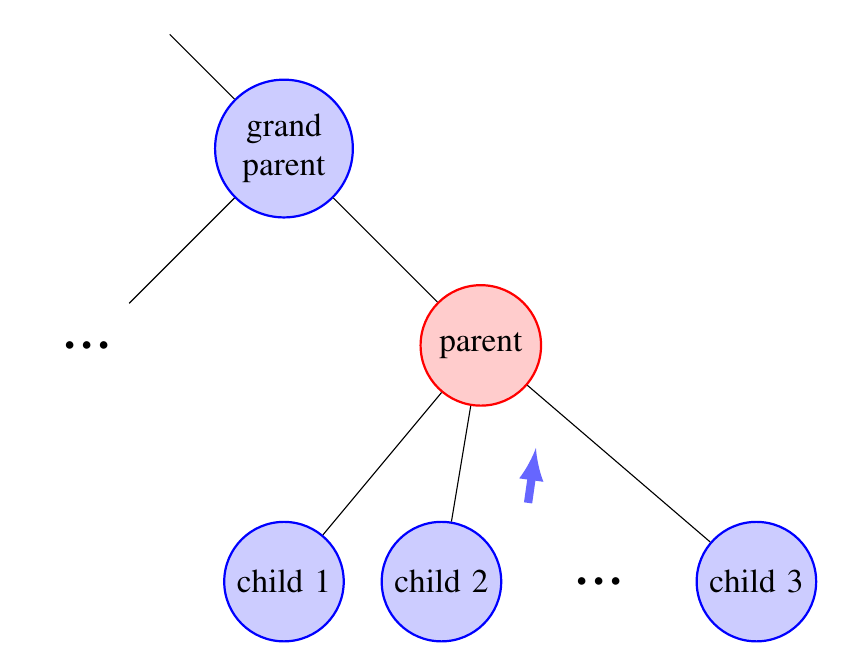
\begin{tikzpicture}[
            every node/.style={
            thick, inner sep=0.1em, text centered, font=\large, text width=4em}
        ]
        \tikzstyle {blue_circ} = [circle, draw=blue, fill=blue!20]
        \tikzstyle {red_circ} = [circle, draw=red, fill=red!20]
        \tikzstyle {blue_border} = [circle, draw=blue!65]
        \tikzstyle {text_box} = [circle, draw=white, text=black]
        
        \node [blue_circ] (gp) at (-2,5.5) {grand parent};
        \node [red_circ] (p) at (0.5,3) {parent};
        \node [blue_circ] (c1) at (-2,0) {child 1};
        \node [blue_circ] (c2) at (0,0) {child 2};
        \node [blue_circ] (c3) at (4,0) {child 3};
        \node [text_box] (sus_1) at (-4.5, 3) {\Huge ...};
        \node [text_box] (sus_2) at (2, 0) {\Huge ...};
        
        \node (left) at (-4.5,3) {};
        \node (root) at (-3.5,7) {};
        
        % \draw  (gp) edge (left);
        \draw  (gp) edge (sus_1);
        \draw  (gp) edge (p);
        \draw  (p) edge (c1);
        \draw  (p) edge (c2);
        \draw  (p) edge (c3);
        \draw  (root) edge (gp);
        
        \draw[-latex, draw=blue!60, line width=3pt] (1.1,1) -- (1.2,1.7);
        
        \end{tikzpicture} 
    }
    \caption{Parent node fails and its children detect the absence.}
    \label{Fig:Missing}
\end{figure}

\begin{figure}[htb]
    \centering
    
    \resizebox{0.8\linewidth}{!}{
        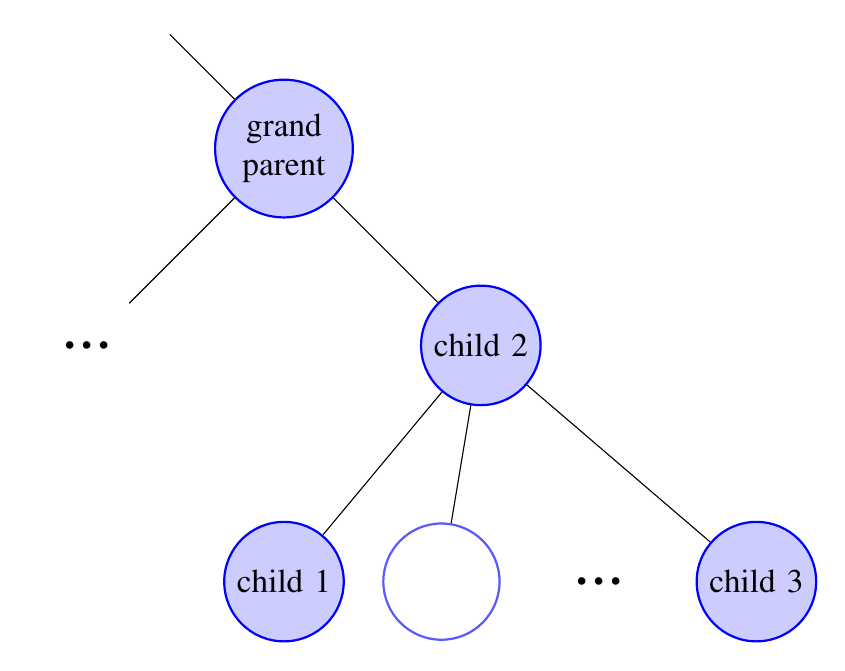
\begin{tikzpicture}[
            every node/.style={
            thick, inner sep=0.1em, text centered, font=\large, text width=4em}
        ]
        \tikzstyle {blue_circ} = [circle, draw=blue, fill=blue!20]
        \tikzstyle {red_circ} = [circle, draw=red, fill=red!20]
        \tikzstyle {blue_border} = [circle, draw=blue!65]
        \tikzstyle {text_box} = [circle, draw=white, text=black]
        
        \node [blue_circ] (gp) at (-2,5.5) {grand parent};
        \node [blue_circ] (p) at (0.5,3) {child 2};
        \node [blue_circ] (c1) at (-2,0) {child 1};
        \node [blue_border] (c2) at (0,0) {};
        \node [blue_circ] (c3) at (4,0) {child 3};
        \node [text_box] (sus_1) at (-4.5, 3) {\Huge ...};
        \node [text_box] (sus_2) at (2, 0) {\Huge ...};
        
        \node (left) at (-4.5,3) {};
        \node (root) at (-3.5,7) {};
        
        \draw  (gp) edge (sus_1);
        \draw  (gp) edge (p);
        \draw  (p) edge (c1);
        \draw  (p) edge (c2);
        \draw  (p) edge (c3);
        \draw  (root) edge (gp);
    	
        \end{tikzpicture}
    }
    
    \caption{Child 2 was elected the oldest and replaced the missing parent}
    \label{Fig:Replacement}
\end{figure}

Next, we describe a solution to improve the protection of the botnet against this kind of security systems. If a node detects that its parent is missing, it should start the election process to decide a new one. In the adopted 
strategy, as exemplified in the Figures \ref{Fig:Missing} and \ref{Fig:Replacement}, the oldest child of the missing parent takes its place.

However, the timestamp on the system clock, when the zombie joined the botnet, is used  to compare the zombie nodes and to decide who is the oldest brother. This is sufficient to avoid an invader from forging its own time by pretending to be older in order to substitute a missing parent.

\section{\uppercase{Conclusion}} \label{sec:conclusion}

The simulation of DDoS mechanisms implemented in this work could obtain interesting results preserving the functionality of a real DDoS and clarifying the dissemination of information within a botnet along with its interacting behavior.

As described in the previous sections, the list-based implementation could expose the differences in each ARD mechanism, since it generates many levels of hierarchy in the topology using a relatively small number of nodes. Thus, phenomena as the network propagation delay can be noticed easier: the time to mobilize all bots in the network is more expressive and the two mechanisms of attack generate very different results.

In terms of package loss in the targeted system, both mechanisms (Continuous streaming and Pulsating waves) generated similar outputs. This is expected for a limited target infrastructure and can be interpreted as the botnet having more network bandwidth capacity than the target.

We also propose a new election strategy to manage the dynamic structure of the botnet network, when zombie nodes detect failed parents, improving the security against mitigation by security systems. The proposed method theoretically meets the objective of preventing the botnet mitigation by outside invaders. However, since the simulation of a real scenario of security system attacking botnets is not trivial, we preferred to explore such simulations in future projects. 

Finally, since DDoS from the attacker perspective is not a common topic in the academia, we expect this work helps to improve this discussion and can be used as material to new computer network and distributed system courses.





%\vfill

\bibliographystyle{apalike}
{\small
\bibliography{ddos}}

\end{document}